\documentclass[]{article}
\usepackage{lmodern}
\usepackage{amssymb,amsmath}
\usepackage{ifxetex,ifluatex}
\usepackage{fixltx2e} % provides \textsubscript
\ifnum 0\ifxetex 1\fi\ifluatex 1\fi=0 % if pdftex
  \usepackage[T1]{fontenc}
  \usepackage[utf8]{inputenc}
\else % if luatex or xelatex
  \ifxetex
    \usepackage{mathspec}
  \else
    \usepackage{fontspec}
  \fi
  \defaultfontfeatures{Ligatures=TeX,Scale=MatchLowercase}
\fi
% use upquote if available, for straight quotes in verbatim environments
\IfFileExists{upquote.sty}{\usepackage{upquote}}{}
% use microtype if available
\IfFileExists{microtype.sty}{%
\usepackage{microtype}
\UseMicrotypeSet[protrusion]{basicmath} % disable protrusion for tt fonts
}{}
\usepackage[margin=1in]{geometry}
\usepackage{hyperref}
\hypersetup{unicode=true,
            pdfborder={0 0 0},
            breaklinks=true}
\urlstyle{same}  % don't use monospace font for urls
\usepackage{longtable,booktabs}
\usepackage{graphicx}
% grffile has become a legacy package: https://ctan.org/pkg/grffile
\IfFileExists{grffile.sty}{%
\usepackage{grffile}
}{}
\makeatletter
\def\maxwidth{\ifdim\Gin@nat@width>\linewidth\linewidth\else\Gin@nat@width\fi}
\def\maxheight{\ifdim\Gin@nat@height>\textheight\textheight\else\Gin@nat@height\fi}
\makeatother
% Scale images if necessary, so that they will not overflow the page
% margins by default, and it is still possible to overwrite the defaults
% using explicit options in \includegraphics[width, height, ...]{}
\setkeys{Gin}{width=\maxwidth,height=\maxheight,keepaspectratio}
\IfFileExists{parskip.sty}{%
\usepackage{parskip}
}{% else
\setlength{\parindent}{0pt}
\setlength{\parskip}{6pt plus 2pt minus 1pt}
}
\setlength{\emergencystretch}{3em}  % prevent overfull lines
\providecommand{\tightlist}{%
  \setlength{\itemsep}{0pt}\setlength{\parskip}{0pt}}
\setcounter{secnumdepth}{0}
% Redefines (sub)paragraphs to behave more like sections
\ifx\paragraph\undefined\else
\let\oldparagraph\paragraph
\renewcommand{\paragraph}[1]{\oldparagraph{#1}\mbox{}}
\fi
\ifx\subparagraph\undefined\else
\let\oldsubparagraph\subparagraph
\renewcommand{\subparagraph}[1]{\oldsubparagraph{#1}\mbox{}}
\fi

%%% Use protect on footnotes to avoid problems with footnotes in titles
\let\rmarkdownfootnote\footnote%
\def\footnote{\protect\rmarkdownfootnote}

%%% Change title format to be more compact
\usepackage{titling}

% Create subtitle command for use in maketitle
\providecommand{\subtitle}[1]{
  \posttitle{
    \begin{center}\large#1\end{center}
    }
}

\setlength{\droptitle}{-2em}

  \title{}
    \pretitle{\vspace{\droptitle}}
  \posttitle{}
    \author{}
    \preauthor{}\postauthor{}
    \date{}
    \predate{}\postdate{}
  

\begin{document}

\hypertarget{group-presentation-order}{%
\subsection{Group Presentation Order}\label{group-presentation-order}}

\begin{verbatim}
##                                  group_name order  day
## 1                                       VAR     1 12/3
## 2                Property Rights and Wrongs     2 12/3
## 3                                Cool_Group     3 12/3
## 4                             Pink Gorrilaz     4 12/3
## 5                                       CCT     5 12/3
## 6                                Carbon Tax     6 12/3
## 7                             We Love James     7 12/3
## 8                             The Windmills     8 12/3
## 9                               Vroom Vroom     9 12/6
## 10            Judges for Endangered Species    10 12/6
## 11                               Protectors    11 12/6
## 12 Student Coalition for the Green New Deal    12 12/6
\end{verbatim}

\hypertarget{section}{%
\subsection{}\label{section}}

Whiskey is for drinking; water is for fighting over. -Mark Twain

When the well's dry, we know the worth of water. -Benjamin Franklin

\hypertarget{section-1}{%
\subsection{}\label{section-1}}

So far in this class we have talked about:

\begin{itemize}
\tightlist
\item
  Environmental Externality

  \begin{itemize}
  \tightlist
  \item
    Pollution control
  \end{itemize}
\item
  Property Rights Regimes

  \begin{itemize}
  \tightlist
  \item
    Exclusivity, Rivalry, and Transferability
  \end{itemize}
\item
  Scarcity

  \begin{itemize}
  \tightlist
  \item
    What measures economic scarcity
  \item
    What happens when market cannot deliver the signal of scarcity
  \end{itemize}
\end{itemize}

\hypertarget{in-this-module-we-will-talk-about}{%
\subsection{In this module we will talk
about:}\label{in-this-module-we-will-talk-about}}

\begin{itemize}
\tightlist
\item
  What are we talking about when we talk about water?
\item
  Water quantity

  \begin{itemize}
  \tightlist
  \item
    Who is using the water?
  \item
    Who owns the water?
  \item
    How to allocate water?
  \end{itemize}
\item
  Water quality

  \begin{itemize}
  \tightlist
  \item
    Sanitation
  \item
    Pollution
  \end{itemize}
\end{itemize}

\hypertarget{section-2}{%
\subsection{}\label{section-2}}

\hypertarget{section-3}{%
\subsection{}\label{section-3}}

\begin{itemize}
\tightlist
\item
  Only a tiny fraction of the earth's water can be used

  \begin{itemize}
  \tightlist
  \item
    0.3\% of the water feeds 7 billion people
  \end{itemize}
\item
  750 million people lacks clean water

  \begin{itemize}
  \tightlist
  \item
    Drinking dirty water leads to a series of diseases, or even death
  \end{itemize}
\item
  A drop of water is worth more than a sack of gold to a thirsty man
\end{itemize}

\hypertarget{section-4}{%
\subsection{}\label{section-4}}

When we ``conserve'' water, what are we really conserving?

Or, what is the harm of ``wasting'' water?

\hypertarget{two-fundamentally-different-challenges}{%
\subsection{Two fundamentally different
challenges}\label{two-fundamentally-different-challenges}}

\begin{itemize}
\tightlist
\item
  Water quantity problem

  \begin{itemize}
  \tightlist
  \item
    Not enough water to suffice human need
  \item
    Cape Cod, California, Dubai, Israel
  \item
    A resource problem: property rights
  \end{itemize}
\item
  Water quality problem

  \begin{itemize}
  \tightlist
  \item
    Water is not clean enough to drink/use/recreate
  \item
    Charles River, Potomac, Yangtze, Ganges
  \item
    An environmental problem: externality
  \end{itemize}
\end{itemize}

\hypertarget{section-5}{%
\subsection{}\label{section-5}}

\begin{enumerate}
\def\labelenumi{\arabic{enumi}.}
\tightlist
\item
  From your perspective, at what point (if any) does this discussion
  about water rights break down or become irrelevant for the Western
  US?\\
\item
  How do dramatic technical innovations fit into the economic
  assessment? What is the probability of the implementation of
  approaches that are currently considered `wild' (for example, piping
  water from Canada and/or Alaska, large scale desalination factories
  and piping from the west, etc). At what point (if ever) do these
  become feasible?
\end{enumerate}

\hypertarget{section-6}{%
\subsection{}\label{section-6}}

\begin{enumerate}
\def\labelenumi{\arabic{enumi}.}
\setcounter{enumi}{2}
\tightlist
\item
  At the moment, there are clear winners and losers in the water rights
  systems of the western states. What would happen to the system if a
  technological solution were found (and implemented) that removed the
  concern about water supply in the region?
\end{enumerate}

\hypertarget{water-as-a-resource}{%
\subsection{Water as a resource}\label{water-as-a-resource}}

\begin{itemize}
\tightlist
\item
  Surface water is a renewable resource consisting of rivers, lakes, and
  reservoirs.
\item
  Groundwater is water that collects underground in aquifers.

  \begin{itemize}
  \tightlist
  \item
    Some aquifers are non-recharging and are thus nonrenewable resources
  \item
    Others could potentially be recharged if hydraulically connected
    with a surface water system
  \end{itemize}
\end{itemize}

\hypertarget{section-7}{%
\subsection{}\label{section-7}}

\begin{itemize}
\tightlist
\item
  Many places in the world is facing water challenges

  \begin{itemize}
  \tightlist
  \item
    4 Billion people is under stress at least seasonally
  \item
    Half of them live in India or China
  \end{itemize}
\item
  Supply of water

  \begin{itemize}
  \tightlist
  \item
    Surface water
  \item
    Groundwater
  \end{itemize}
\item
  Demand for water

  \begin{itemize}
  \tightlist
  \item
    Population
  \item
    Water usage patterns
  \end{itemize}
\end{itemize}

\hypertarget{drought-has-been-particularly-challenging}{%
\subsection{Drought has been particularly
challenging}\label{drought-has-been-particularly-challenging}}

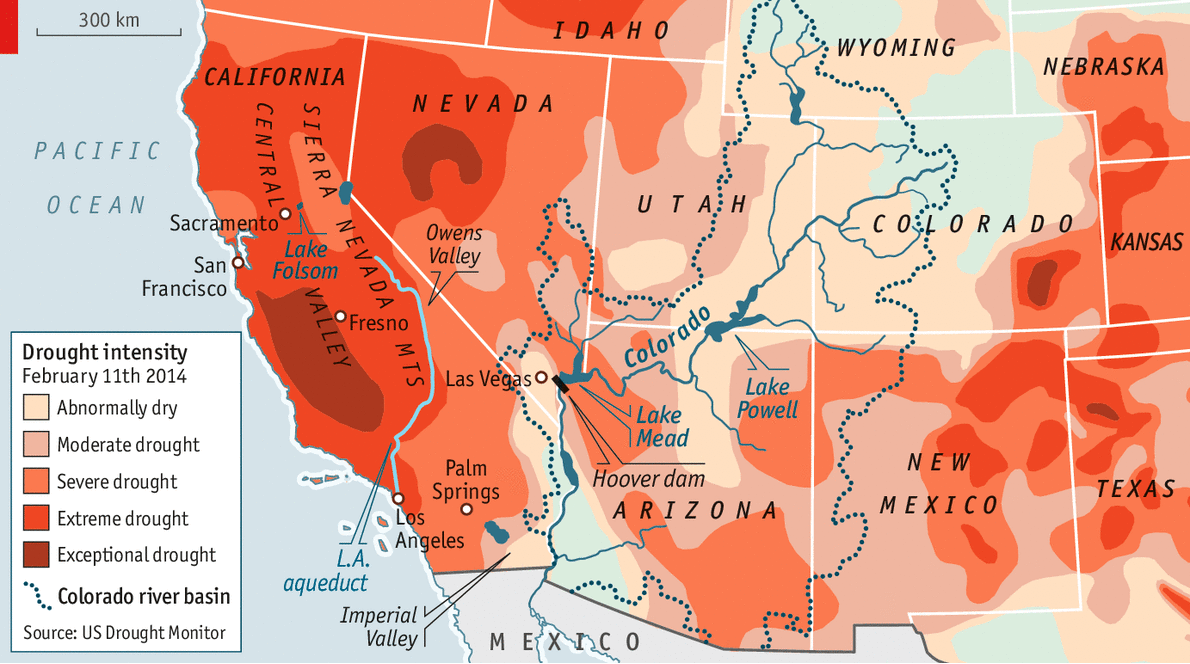
\includegraphics[width=\textwidth,height=4.16667in]{figures/m10_drought_in_the_west.png}

\hypertarget{section-8}{%
\subsection{}\label{section-8}}

\includegraphics[width=\textwidth,height=4.16667in]{figures/m10_hoover_dam.jpg}

\hypertarget{section-9}{%
\subsection{}\label{section-9}}

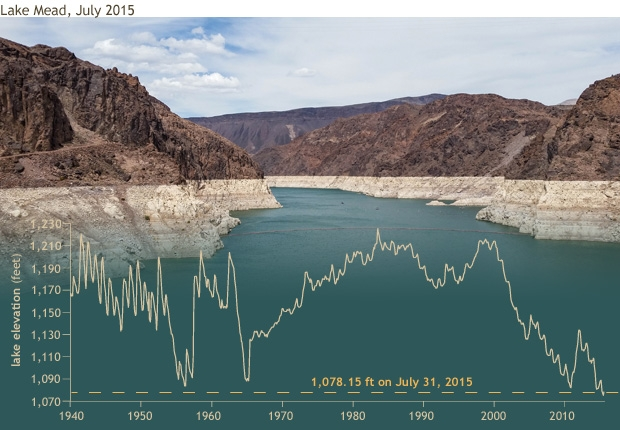
\includegraphics[width=\textwidth,height=4.16667in]{figures/m10_lake_mead_level.jpg}

\hypertarget{section-10}{%
\subsection{}\label{section-10}}

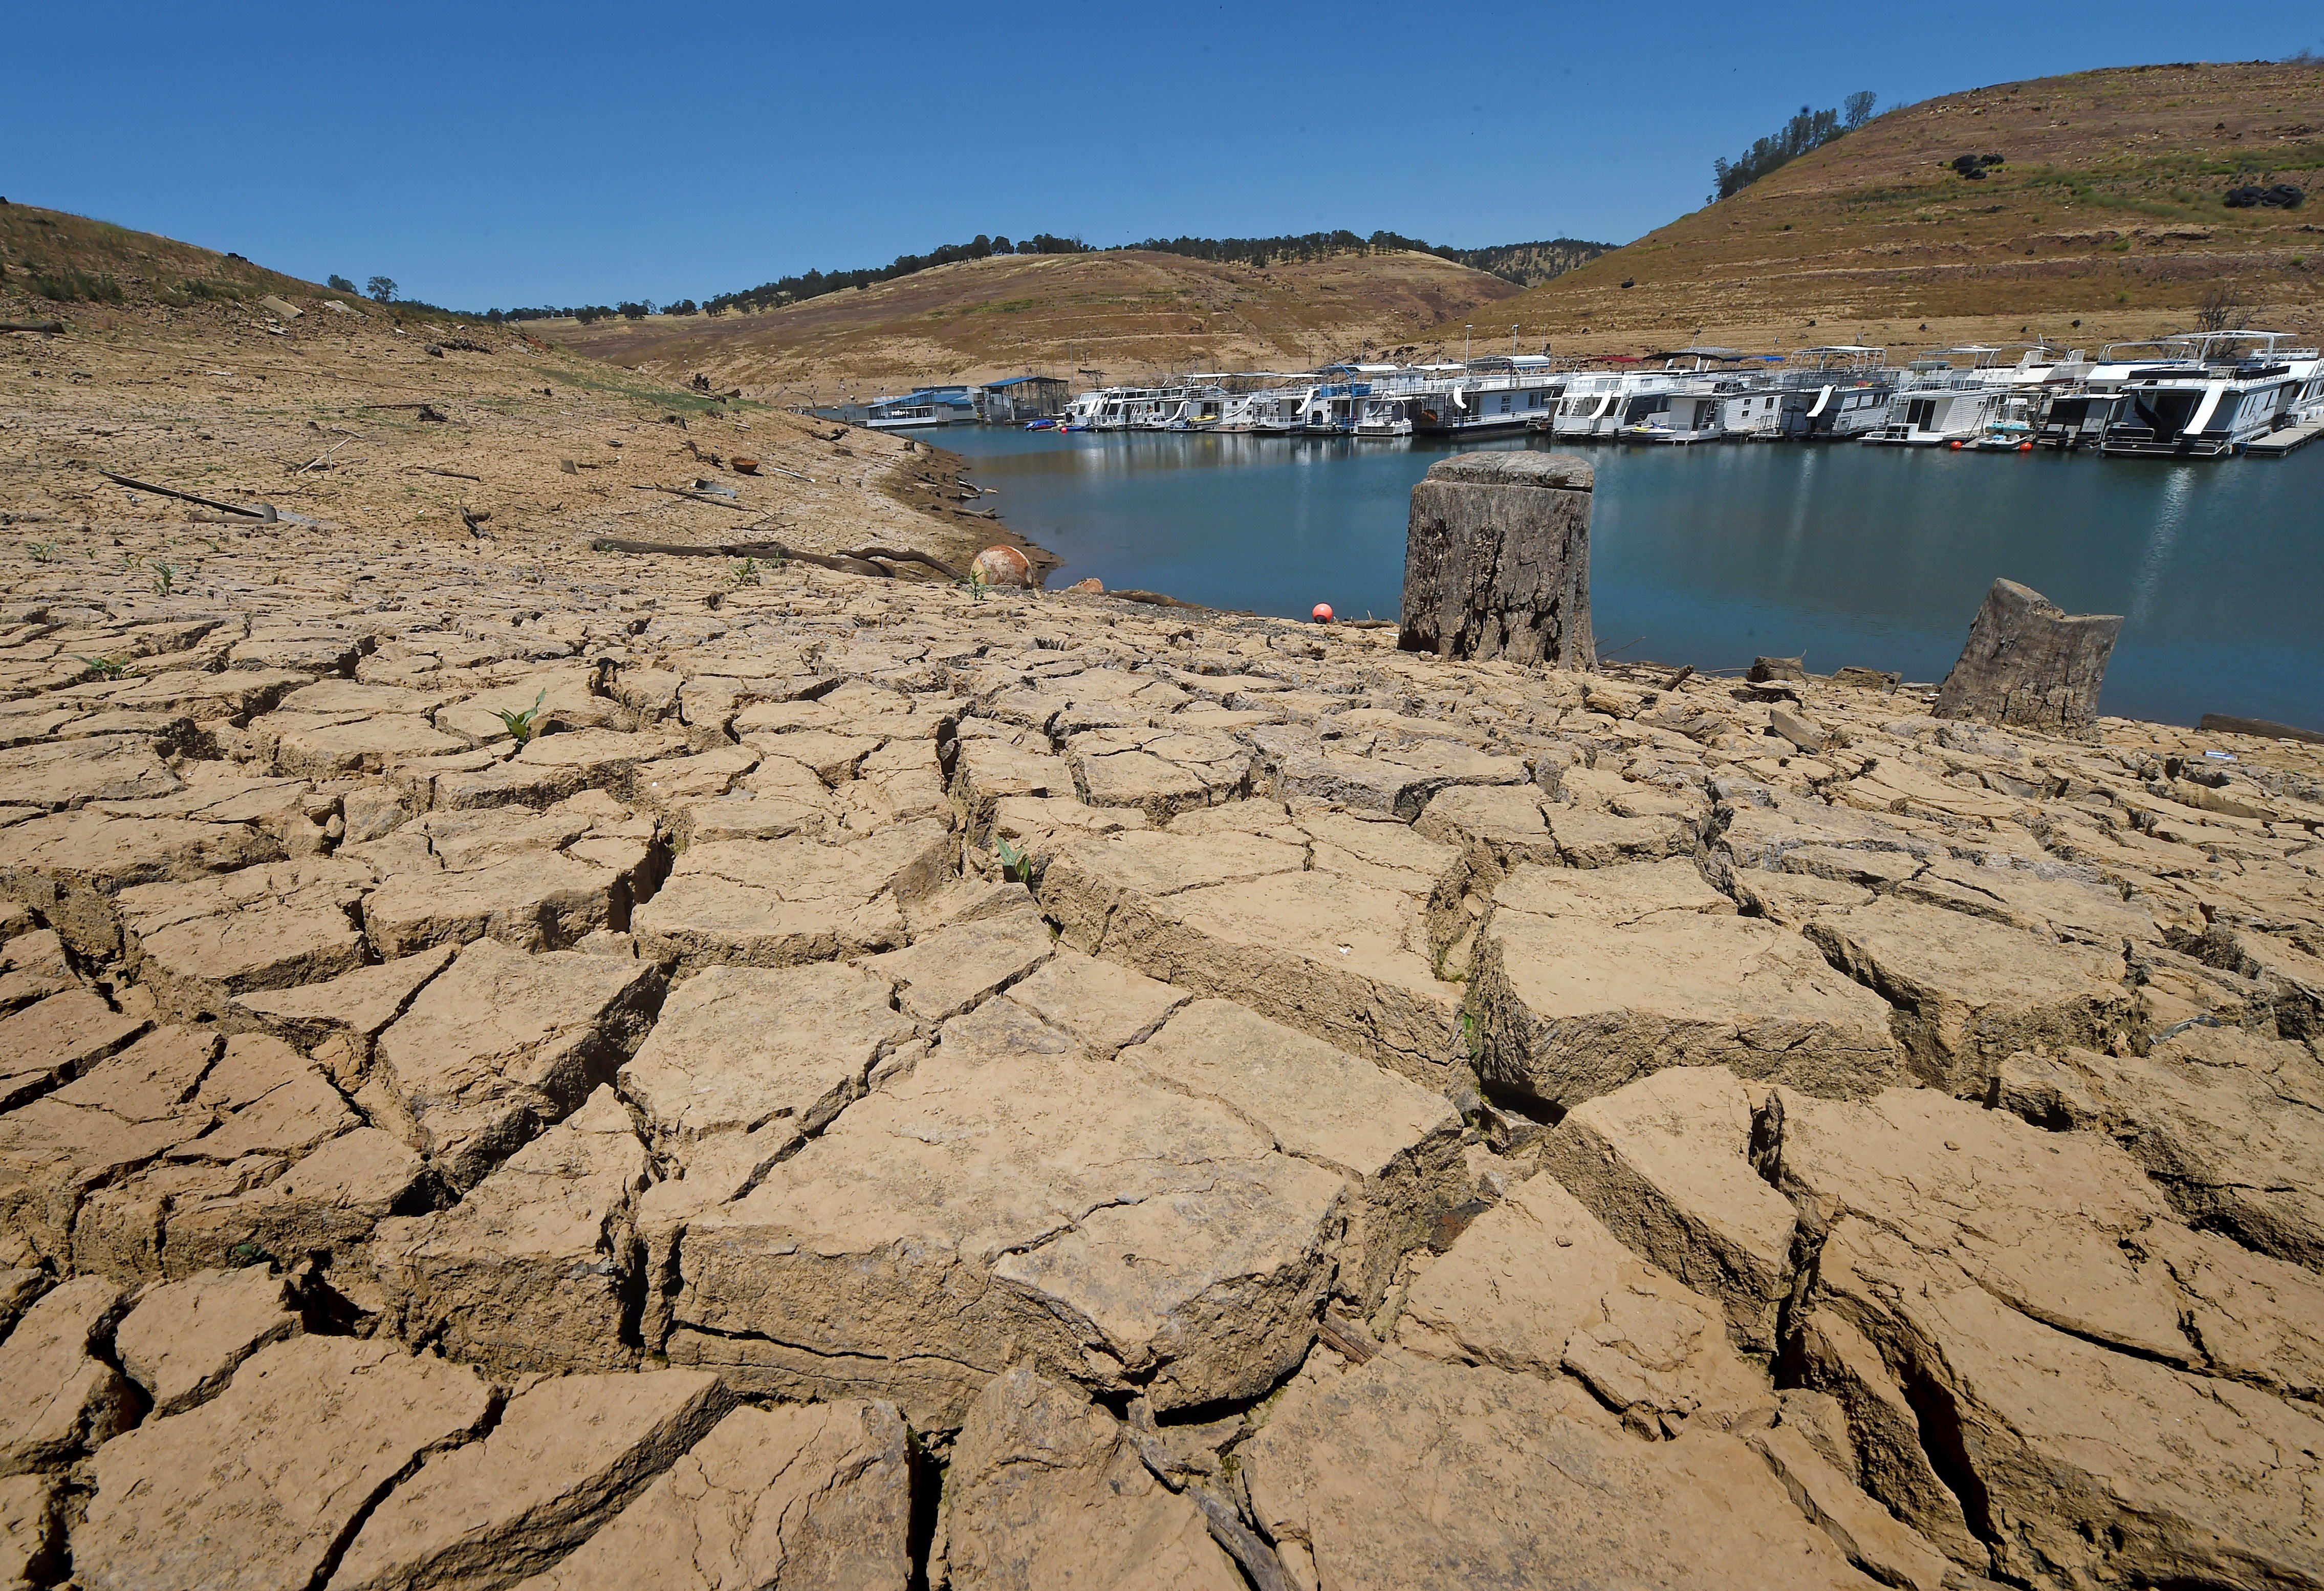
\includegraphics[width=\textwidth,height=4.16667in]{figures/m10_california_drought.jpg}

\hypertarget{section-11}{%
\subsection{}\label{section-11}}

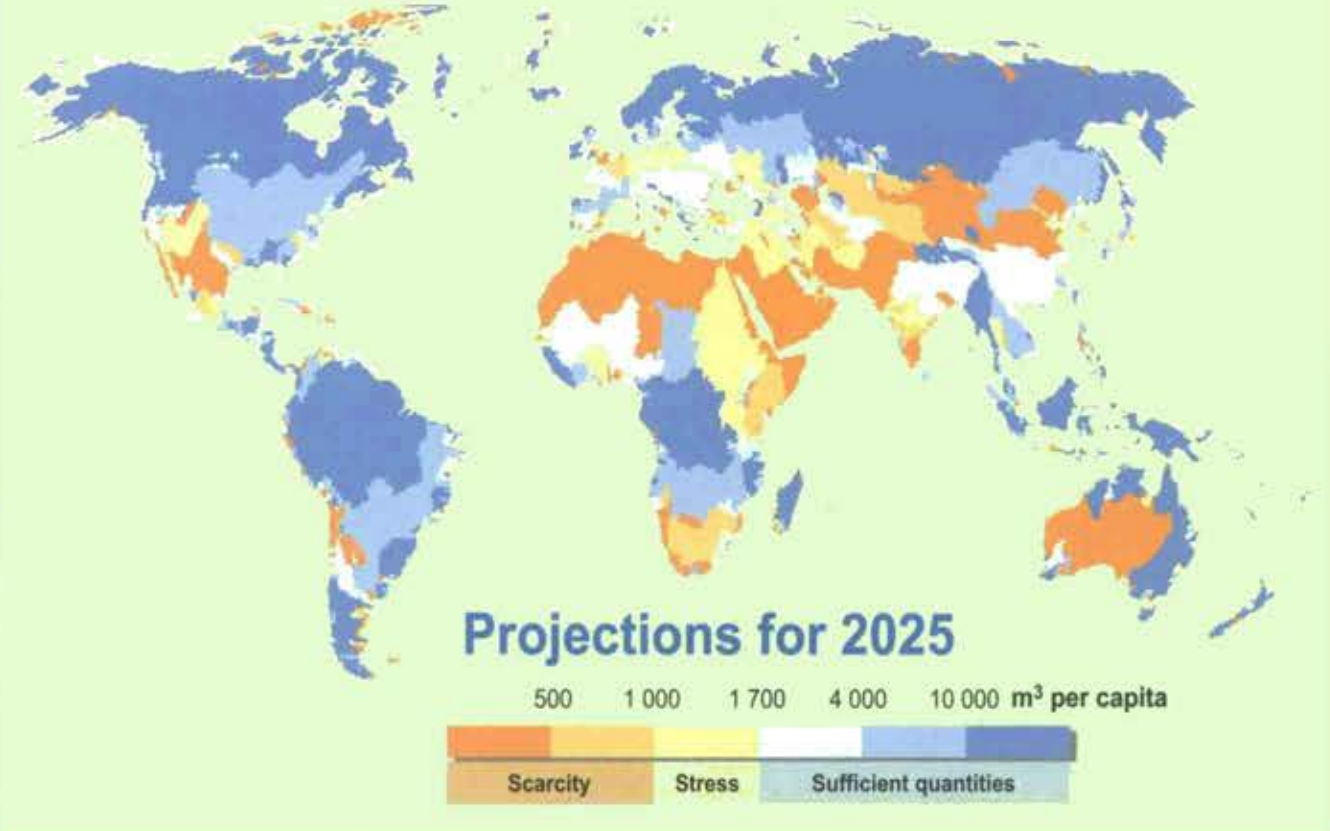
\includegraphics[width=\textwidth,height=4.16667in]{figures/m10_freshwater_per_capita.png}

\hypertarget{section-12}{%
\subsection{}\label{section-12}}

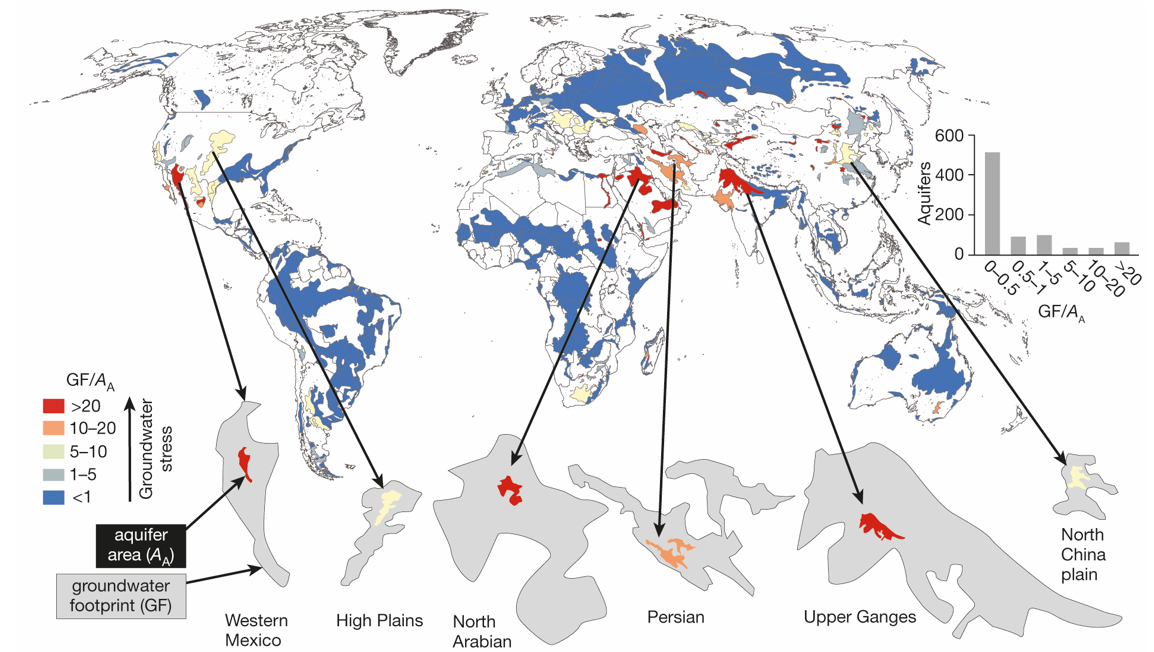
\includegraphics[width=\textwidth,height=4.16667in]{figures/m10_groundwater_availability.png}

\hypertarget{section-13}{%
\subsection{}\label{section-13}}

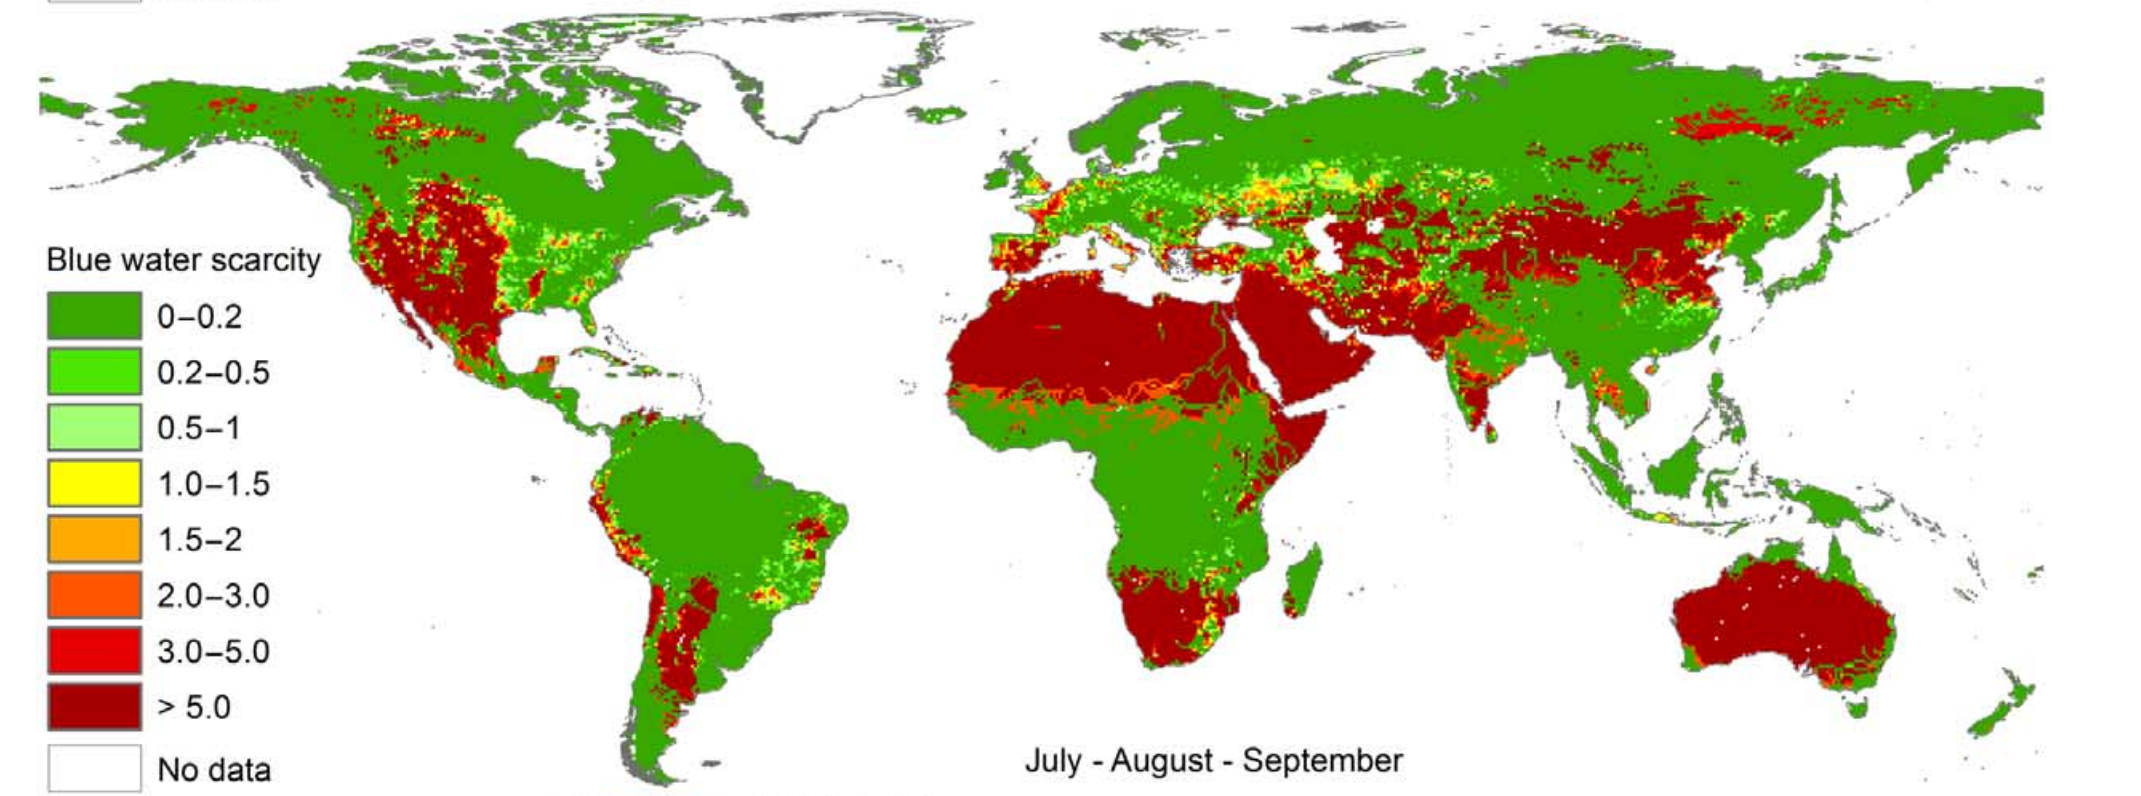
\includegraphics[width=\textwidth,height=3.64583in]{figures/m10_blue_water_scarcity.png}

\hypertarget{section-14}{%
\subsection{}\label{section-14}}

\begin{itemize}
\tightlist
\item
  Everything till now is ``physical scarcity''
\item
  Or rather, a simple way of relating ``reserves'' to ``production''

  \begin{itemize}
  \tightlist
  \item
    Many people, little water - water stress
  \item
    Few people, much water - water abundance
  \end{itemize}
\end{itemize}

What can we tell, and what needs to be figured out from this analysis?

\hypertarget{the-economic-problem}{%
\subsection{The Economic Problem}\label{the-economic-problem}}

\begin{itemize}
\tightlist
\item
  The Demand side problem:

  \begin{itemize}
  \tightlist
  \item
    Every user should have the same ``marginal benefit'' from using
    water
  \item
    Drinking water has the highest utility, followed by domestic use,
    industrial, and lastly agricultural use
  \end{itemize}
\item
  The supply side problem

  \begin{itemize}
  \tightlist
  \item
    Getting water from the cheapest source(s)
  \item
    Move to the ``substitutes'' if price for water is high enough
  \end{itemize}
\end{itemize}

\hypertarget{section-15}{%
\subsection{}\label{section-15}}

\begin{itemize}
\tightlist
\item
  The institutional problem

  \begin{itemize}
  \tightlist
  \item
    What if there is no market signal for scarcity?
  \end{itemize}
\end{itemize}

How many of you pay for a water bill based on volumes?

\hypertarget{who-is-using-water}{%
\subsection{Who is using water?}\label{who-is-using-water}}

\hypertarget{section-16}{%
\subsection{}\label{section-16}}

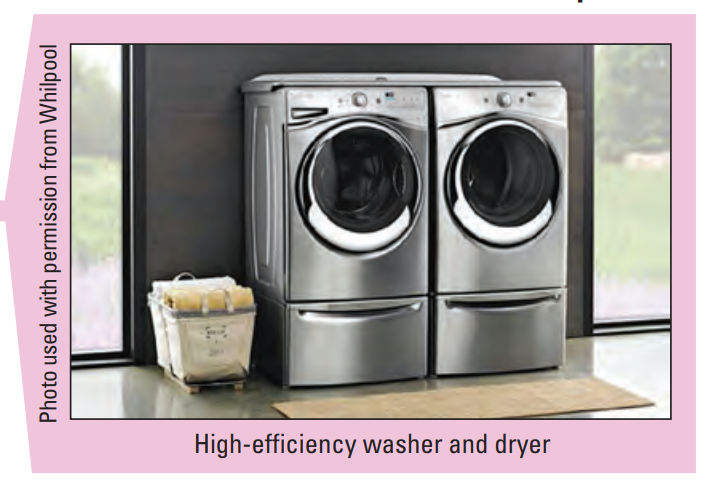
\includegraphics[width=\textwidth,height=4.16667in]{figures/m10_domestic.png}

\hypertarget{section-17}{%
\subsection{}\label{section-17}}

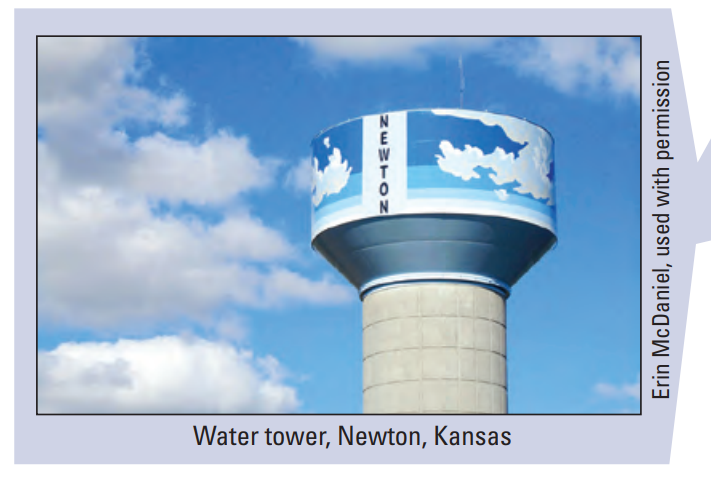
\includegraphics[width=\textwidth,height=4.16667in]{figures/m10_public.png}

\hypertarget{section-18}{%
\subsection{}\label{section-18}}

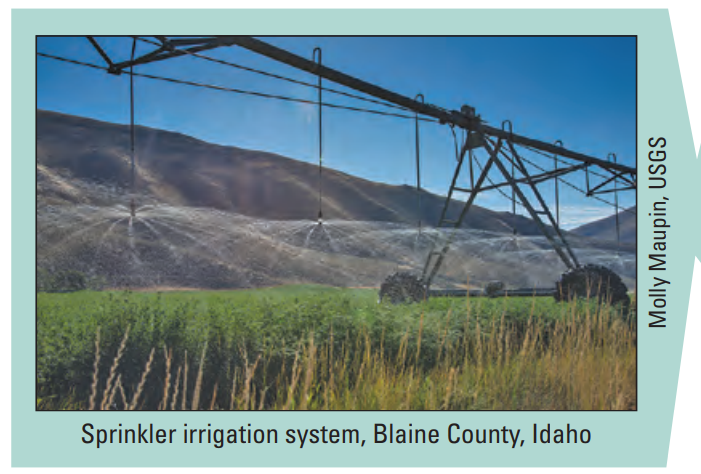
\includegraphics[width=\textwidth,height=4.16667in]{figures/m10_irrigation.png}

\hypertarget{section-19}{%
\subsection{}\label{section-19}}

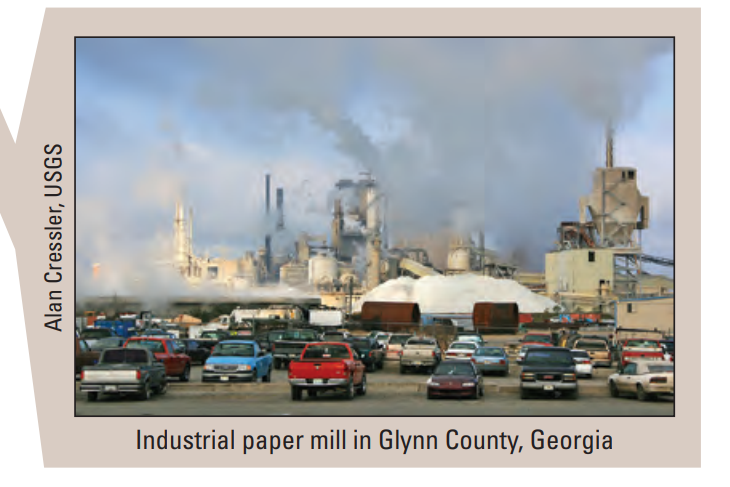
\includegraphics[width=\textwidth,height=4.16667in]{figures/m10_industrial.png}

\hypertarget{section-20}{%
\subsection{}\label{section-20}}

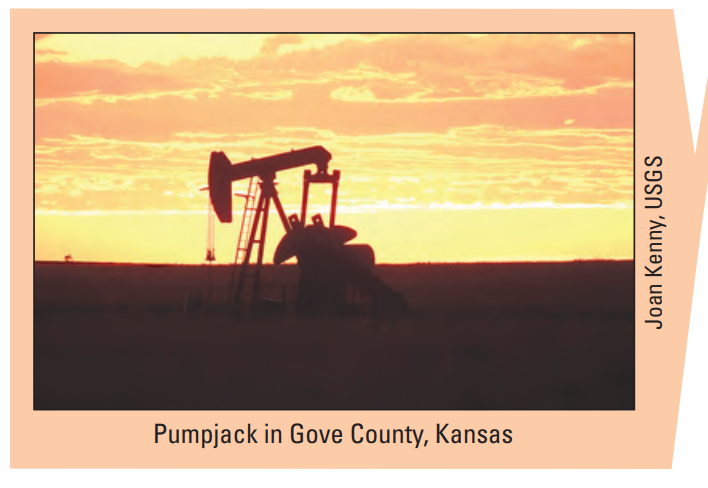
\includegraphics[width=\textwidth,height=4.16667in]{figures/m10_mining.png}

\hypertarget{section-21}{%
\subsection{}\label{section-21}}

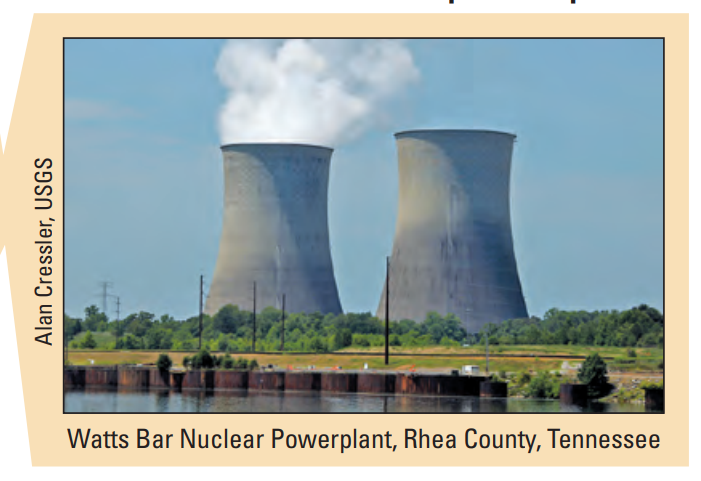
\includegraphics[width=\textwidth,height=4.16667in]{figures/m10_thermal.png}

\hypertarget{who-is-using-water-1}{%
\subsection{Who is using water?}\label{who-is-using-water-1}}

Could you rank the following six sector by their water extraction?

\begin{itemize}
\tightlist
\item
  Domestic
\item
  Other public supply
\item
  Agriculture
\item
  Industrial
\item
  Mining
\item
  Thermoelectric power
\end{itemize}

\hypertarget{water-extraction-in-the-us-year-2010}{%
\subsection{Water extraction in the US, year
2010}\label{water-extraction-in-the-us-year-2010}}

\begin{longtable}[]{@{}ll@{}}
\toprule
Sector & Percentage\tabularnewline
\midrule
\endhead
Thermo power & 45\%\tabularnewline
Agriculture & 37\%\tabularnewline
Domestic & 8\%\tabularnewline
Other Public Supply & 5\%\tabularnewline
Industrial & 4\%\tabularnewline
Mining & 1\%\tabularnewline
\bottomrule
\end{longtable}

\hypertarget{section-22}{%
\subsection{}\label{section-22}}

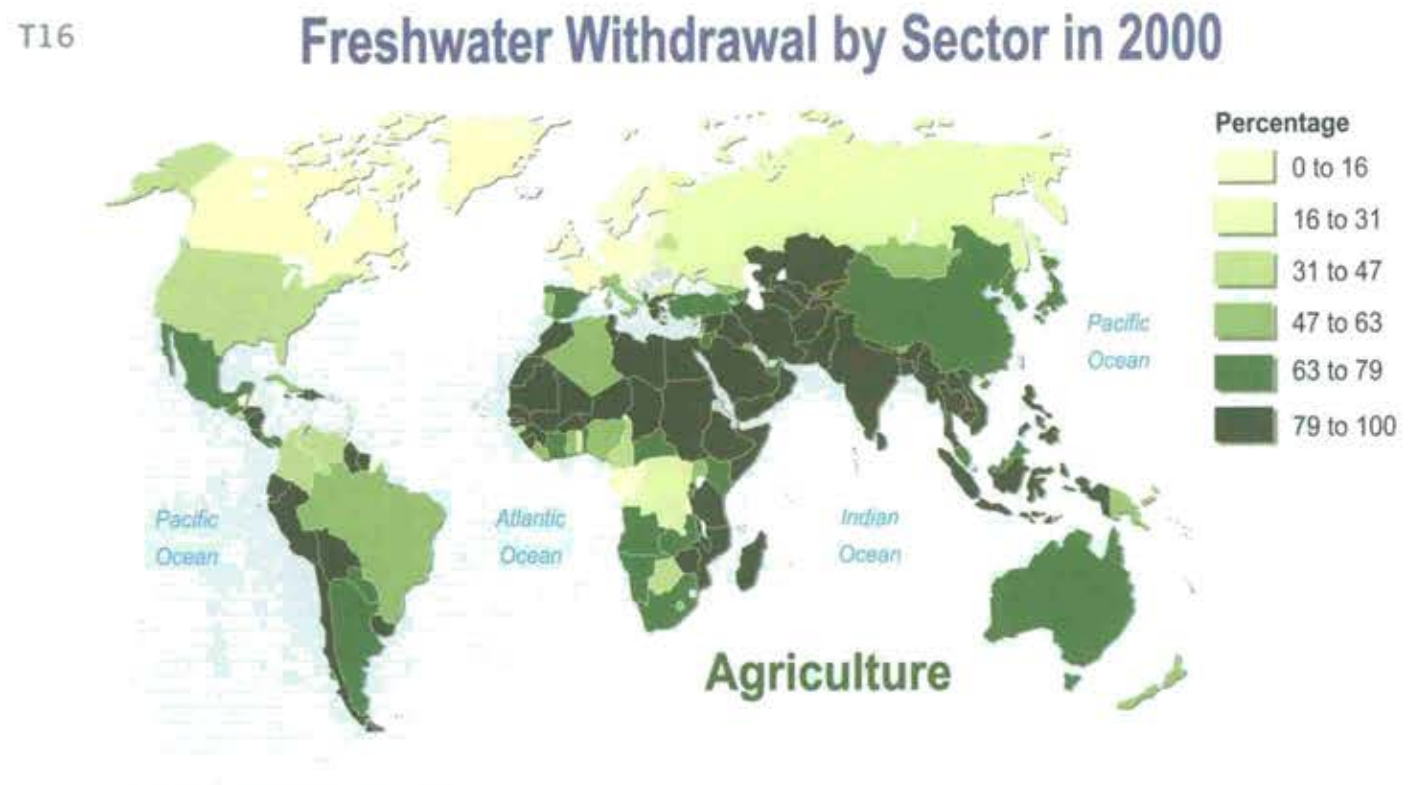
\includegraphics[width=\textwidth,height=4.16667in]{figures/m10_global_agriculture.png}

\hypertarget{section-23}{%
\subsection{}\label{section-23}}

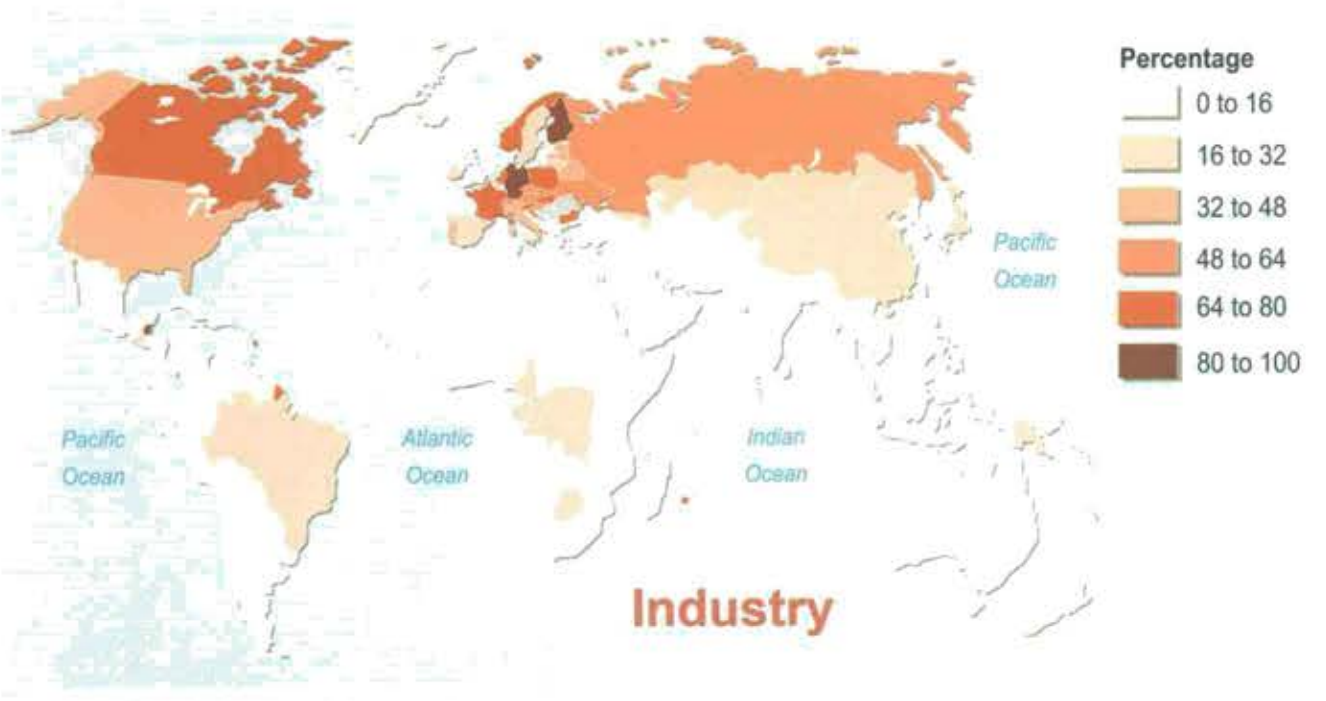
\includegraphics[width=\textwidth,height=4.16667in]{figures/m10_global_industry.png}

\hypertarget{section-24}{%
\subsection{}\label{section-24}}

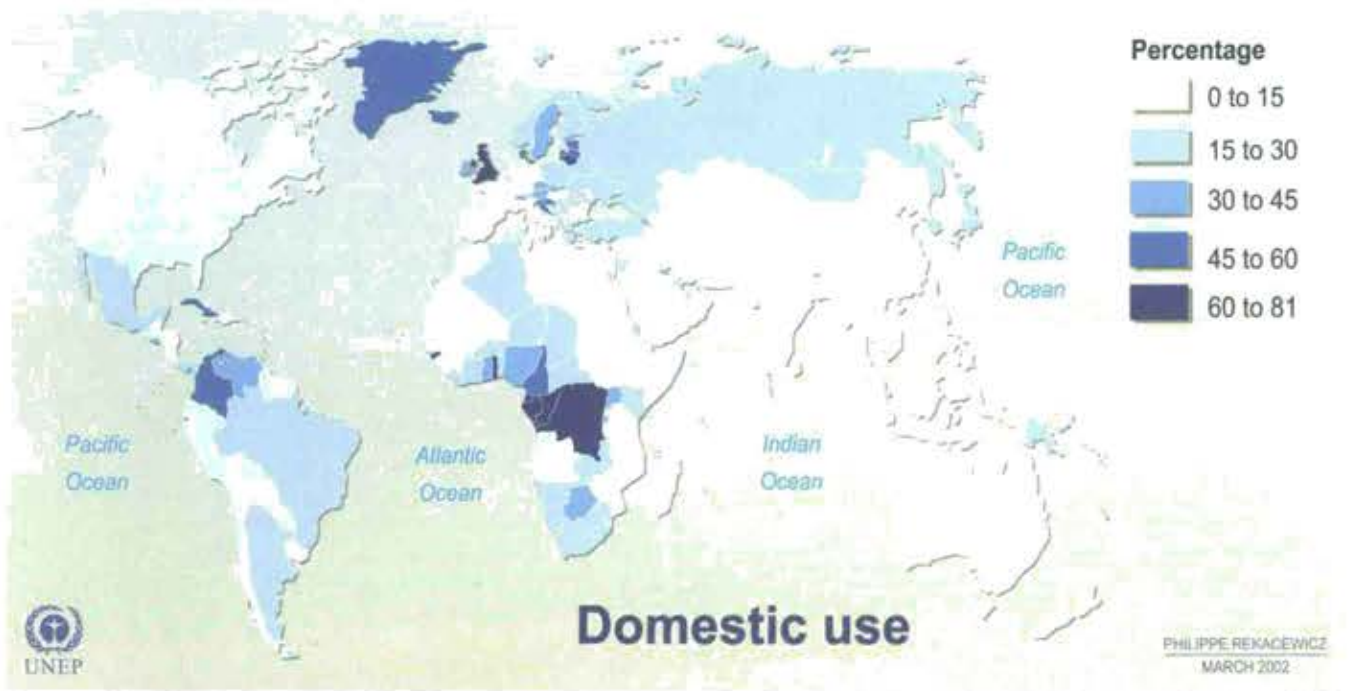
\includegraphics[width=\textwidth,height=4.16667in]{figures/m10_global_domestic.png}

\hypertarget{but-not-all-uses-are-equal}{%
\subsection{But not all uses are
equal}\label{but-not-all-uses-are-equal}}

Why do we complain so much about water used for irrigation, but not for
thermal power generation?

\hypertarget{section-25}{%
\subsection{}\label{section-25}}

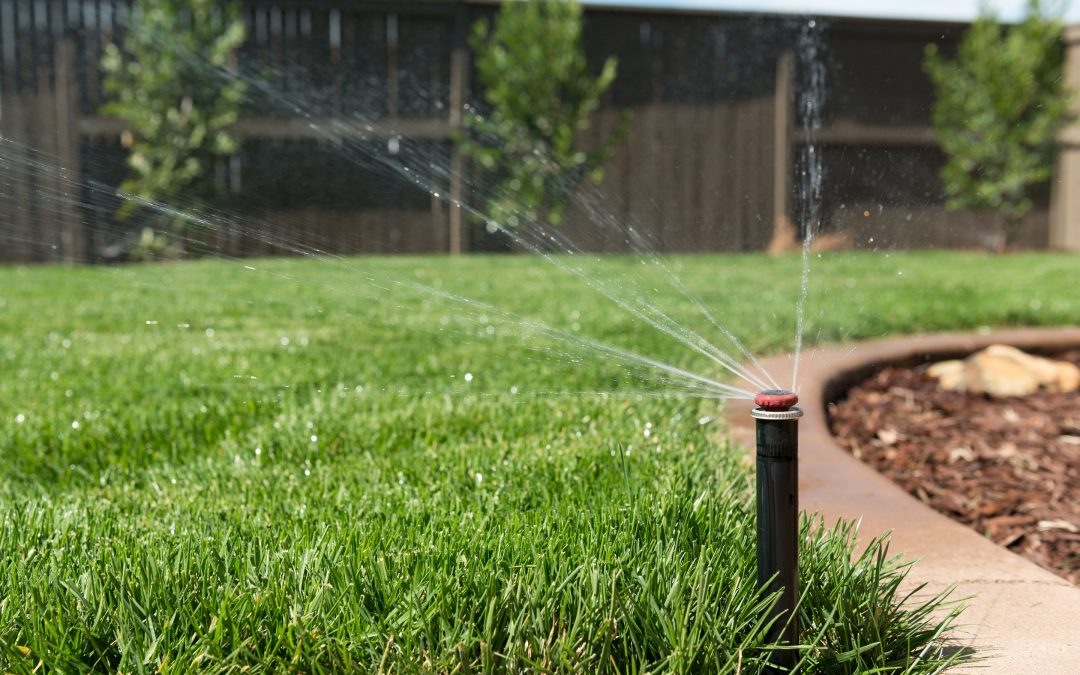
\includegraphics[width=\textwidth,height=4.6875in]{figures/m10_lawn.jpg}

\hypertarget{section-26}{%
\subsection{}\label{section-26}}

\begin{itemize}
\tightlist
\item
  Water extraction (withdraw): amount of water that is taken out from
  the natural water body
\item
  Consumptive use: The part of water withdrawn that is removed from the
  immediate water environment

  \begin{itemize}
  \tightlist
  \item
    Evaporated/transpired
  \item
    Absorbed by crops/products
  \item
    Consumed by humans/livestock
  \end{itemize}
\item
  Return flow (Non-consumptive use): The part of water withdrawn that
  returns to the immediate water environment
\end{itemize}

\hypertarget{section-27}{%
\subsection{}\label{section-27}}

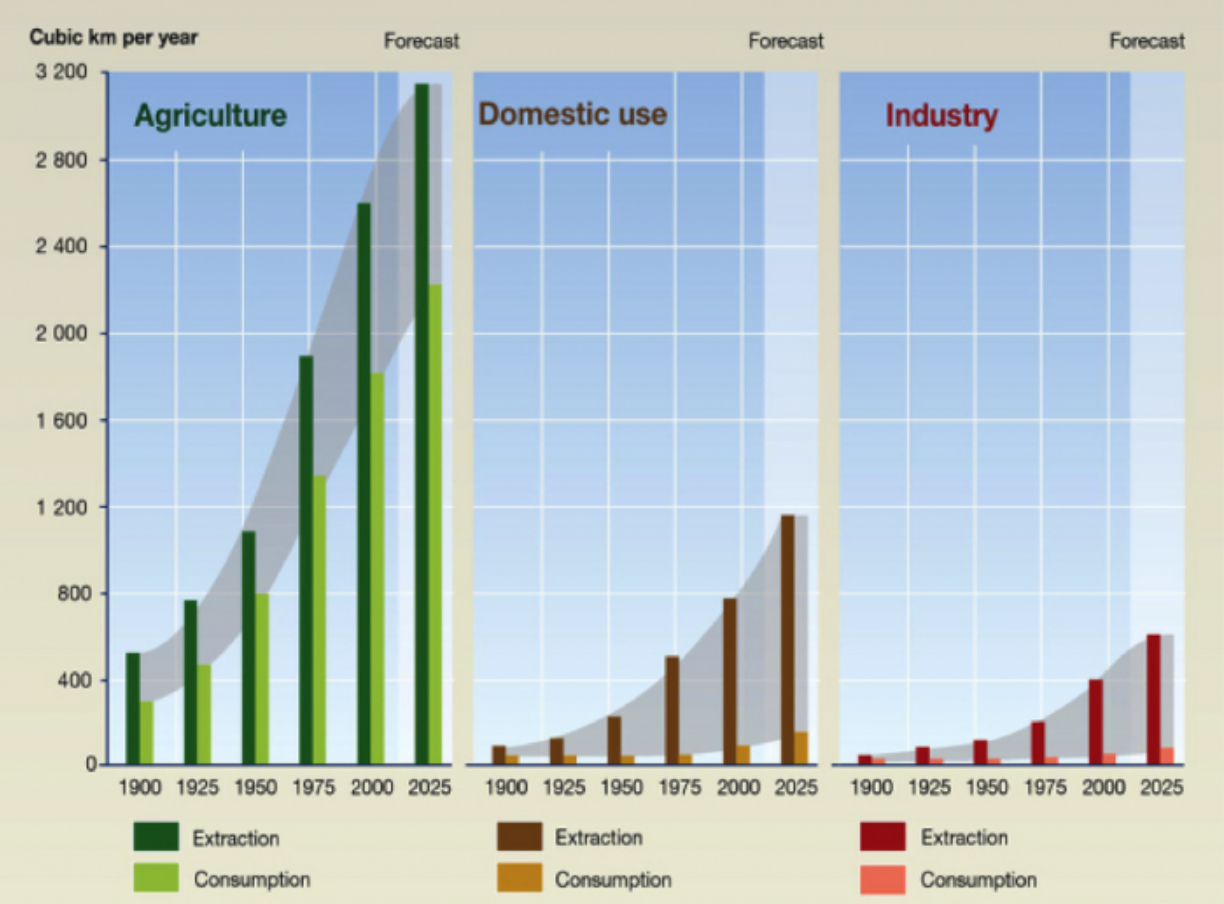
\includegraphics[width=\textwidth,height=4.6875in]{figures/m10_consumptive_use.png}

\hypertarget{section-28}{%
\subsection{}\label{section-28}}

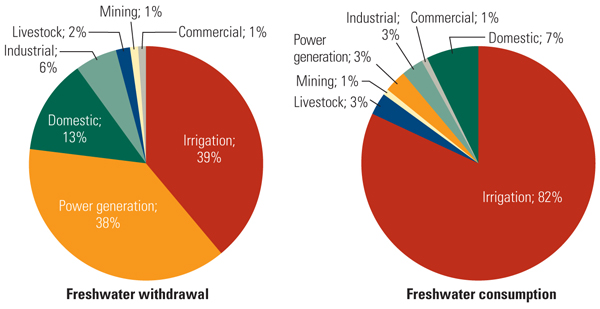
\includegraphics[width=\textwidth,height=4.16667in]{figures/m10_withdraw_vs_consumption.png}

\hypertarget{this-clearly-doesnt-make-sense}{%
\subsection{This clearly doesn't make
sense}\label{this-clearly-doesnt-make-sense}}

At the peak of the California water crisis, restaurant customers have to
pay for tap water. There are limits on how residents can shower.

Meanwhile, farmers in central valley are pouring water on their almonds,
oranges, grapes, etc.

Why is that? Could they simply trade with each other?

\hypertarget{who-owns-water-in-this-country}{%
\subsection{Who owns water in this
country?}\label{who-owns-water-in-this-country}}

Two set of commmon law doctrines govern the legal \textbf{right} to use
surface water

\begin{itemize}
\tightlist
\item
  Riparian doctrine
\item
  Prior appropriation doctrine
\end{itemize}

\hypertarget{section-29}{%
\subsection{}\label{section-29}}

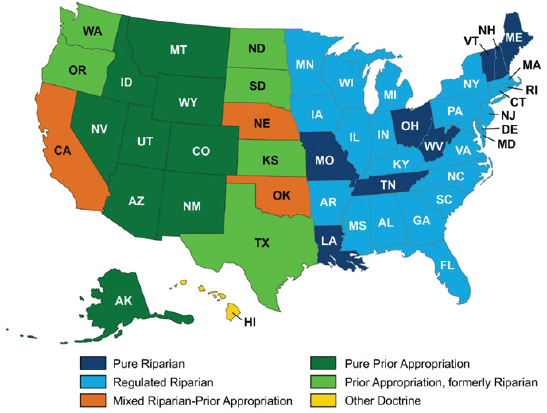
\includegraphics[width=\textwidth,height=4.16667in]{figures/m10_pa_map.jpg}

\hypertarget{section-30}{%
\subsection{}\label{section-30}}

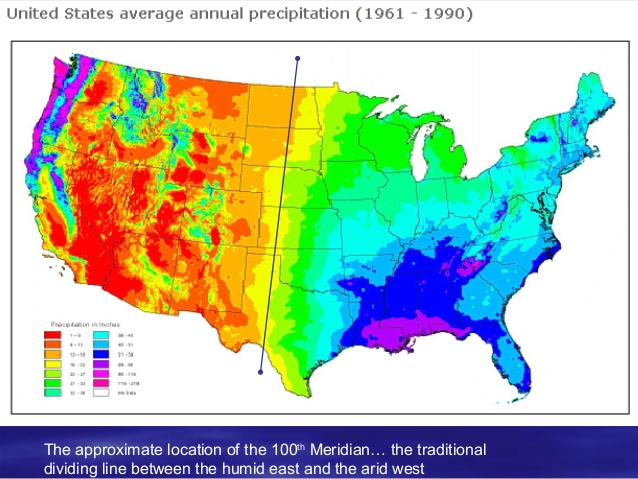
\includegraphics[width=\textwidth,height=4.16667in]{figures/m10_precipitation.jpg}

\hypertarget{the-riparian-doctrine}{%
\subsection{The Riparian Doctrine}\label{the-riparian-doctrine}}

``Anyone who owns property adjacent to the river has a right to use
water''

\begin{itemize}
\tightlist
\item
  ``Riparian'': relating to or situated on the banks of a river
\item
  English Common Law Heritage

  \begin{itemize}
  \tightlist
  \item
    Used in Canada, Australia, Eastern US
  \end{itemize}
\item
  Beneficial use clause: water has to be put into beneficial use
\item
  Non-injury clause: one's use of water should not injury another
  party's capability to use that water
\end{itemize}

\hypertarget{illustration-of-riparian-rights}{%
\subsection{Illustration of Riparian
Rights}\label{illustration-of-riparian-rights}}

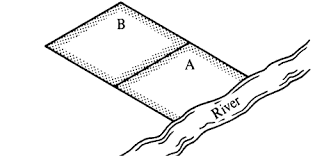
\includegraphics[width=\textwidth,height=4.16667in]{figures/m10_riparian.png}

\hypertarget{type-of-property-rights}{%
\subsection{Type of property rights}\label{type-of-property-rights}}

Does the Riparian doctrine satisfy these characteristics?

\begin{itemize}
\tightlist
\item
  Exclusivity
\item
  Transferability
\item
  Rivalry
\end{itemize}

\hypertarget{section-31}{%
\subsection{}\label{section-31}}

Then why aren't there problems with water resources in most part of the
Eastern US?

\hypertarget{section-32}{%
\subsection{}\label{section-32}}

\hypertarget{the-prior-appropriation-doctrine}{%
\subsection{The Prior Appropriation
Doctrine}\label{the-prior-appropriation-doctrine}}

``First in time, first in rights''

\begin{itemize}
\tightlist
\item
  Anyone who claims to use water first have the right to acquire water
  with priority (seniority)
\item
  In the case of a water shortage, junior water rights will be curtailed
  (cut off) if there is not enough water in the system
\end{itemize}

\hypertarget{additional-provisions-in-the-prior-appropriation-doctrine}{%
\subsection{Additional Provisions in the Prior Appropriation
Doctrine}\label{additional-provisions-in-the-prior-appropriation-doctrine}}

\begin{itemize}
\tightlist
\item
  Beneficial use clause: water has to be put into beneficial use

  \begin{itemize}
  \tightlist
  \item
    As long as one can demonstrate beneficial use, one can apply (and be
    approved) of a reasonable amount of water right
  \end{itemize}
\item
  Usufructuary clause: use it or lose it

  \begin{itemize}
  \tightlist
  \item
    If a right holder no longer uses water, that particular right will
    be (partially or fully) confiscated
  \end{itemize}
\end{itemize}

\hypertarget{sample-of-a-water-right}{%
\subsection{Sample of a water right}\label{sample-of-a-water-right}}

\url{https://www.dropbox.com/s/fprz6f5tarpyibg/Water\%20right\%20examples.pdf?dl=0}

\hypertarget{section-33}{%
\subsection{}\label{section-33}}

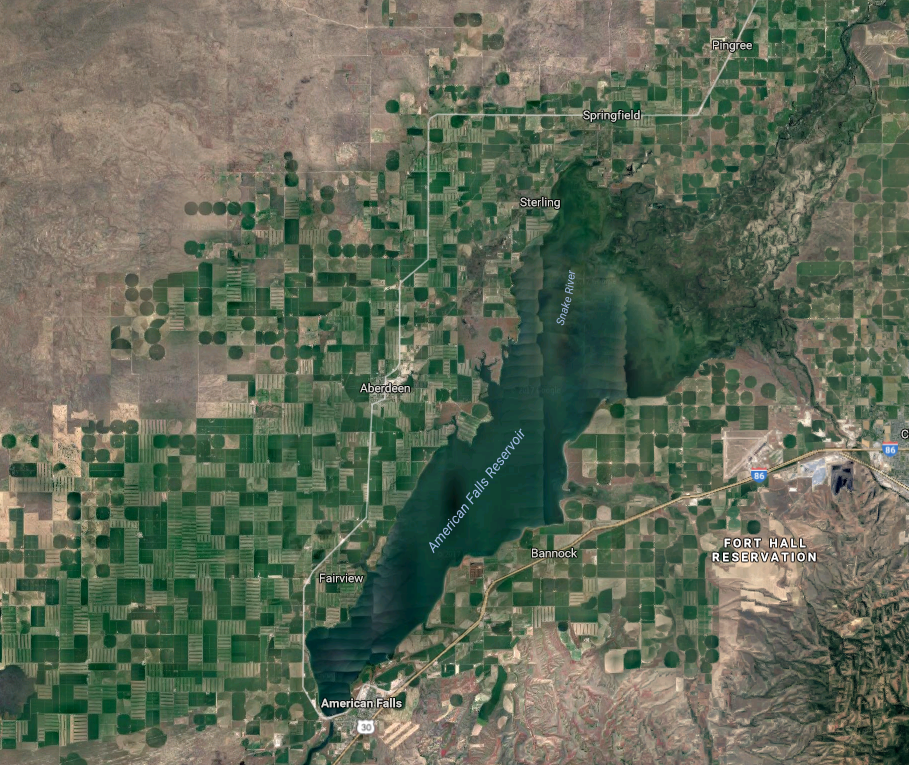
\includegraphics[width=\textwidth,height=4.6875in]{figures/m10_googleearth.png}

\hypertarget{section-34}{%
\subsection{}\label{section-34}}

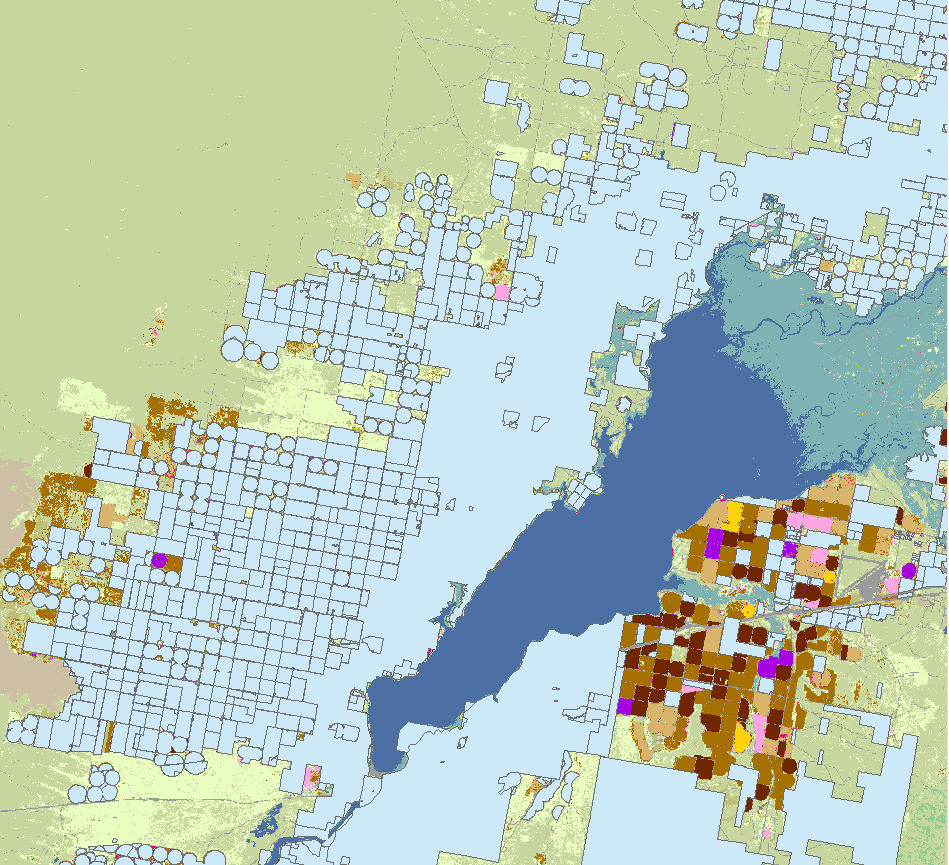
\includegraphics[width=\textwidth,height=4.6875in]{figures/m10_water_rights.png}

\hypertarget{problems-with-prior-appropriation}{%
\subsection{Problems with prior
appropriation}\label{problems-with-prior-appropriation}}

\begin{itemize}
\tightlist
\item
  Water allocation is based on ``seniority''

  \begin{itemize}
  \tightlist
  \item
    If your great grandfather settled at the river basin a year earlier
    than mine, you get the water during a drought and I don't
  \end{itemize}
\item
  Neither an efficient nor a ``just'' allocation system

  \begin{itemize}
  \tightlist
  \item
    Those with junior rights will be completely cut off during a drought
  \item
    (Few) winners and (lots of) losers
  \end{itemize}
\end{itemize}

\hypertarget{section-35}{%
\subsection{}\label{section-35}}

\begin{itemize}
\tightlist
\item
  Coase theorem: if property rights can be traded with zero transaction
  cost, then allocation is still efficient
\item
  Water trades have been extremely hard

  \begin{itemize}
  \tightlist
  \item
    ``Tragedy of the anti-commons''
  \item
    The coordination problem: most water is held by irrigation
    districts, who has to seek consent from all share-holders before
    selling water
  \item
    Third-party effect
  \end{itemize}
\item
  Even trade can happen, transaction costs are high

  \begin{itemize}
  \tightlist
  \item
    ``Water Rights Lawyers''
  \item
    Supreme Court cases
  \end{itemize}
\end{itemize}

\hypertarget{but-why-prior-appropriation}{%
\subsection{But why prior
appropriation?}\label{but-why-prior-appropriation}}

Doesn't the Lincoln-era folks see the problem we face today?

Or, putting it in another way, if you are tasked to design a way to
allocate water in semi-arid part of the world (US West, Northern India,
Northwestern China, or the Middle East), will prior appropriation be
your choice?

Why not assigning water proprotionally?

\hypertarget{a-historical-note}{%
\subsection{A historical note}\label{a-historical-note}}

\begin{itemize}
\tightlist
\item
  When this nation is founded, English common law dominated the legal
  thinking of the founding fathers

  \begin{itemize}
  \tightlist
  \item
    Riparian Law governs water use at that time
  \item
    Think about England in particular: do they have a water shortage
    problem?
  \end{itemize}
\item
  There were abrupt shifts between 1850-1920, from Riparian to Prior
  Appropriation Laws in the Western States

  \begin{itemize}
  \tightlist
  \item
    The Manifest Destiny: the country moved further West to settle
  \item
    Settlers were awarded land as a reward if they could settle in the
    Western lands
  \end{itemize}
\end{itemize}

\hypertarget{section-36}{%
\subsection{}\label{section-36}}

\begin{itemize}
\tightlist
\item
  The settlers quickly figured out that without water, no crop will be
  able to survive in the Western US

  \begin{itemize}
  \tightlist
  \item
    Irrigation is needed
  \end{itemize}
\item
  And the Riparian doctrine won't work so well in the Western US
\end{itemize}

For a couple of reasons. What are they?

\hypertarget{riparian-is-not-the-best-way-to-go}{%
\subsection{Riparian is not the best way to
go}\label{riparian-is-not-the-best-way-to-go}}

Because of the scarce nature of water in the West (and the lack of a
price signal to reflect that)

\begin{itemize}
\tightlist
\item
  Water uses are not quantified
\item
  Only way of exclusion is through land ownership
\item
  Discouraged settling further into lands that are far away from the
  river

  \begin{itemize}
  \tightlist
  \item
    Many lands more fertile than riparian lands with access to
    irrigation water
  \end{itemize}
\end{itemize}

\hypertarget{prior-appropriation}{%
\subsection{Prior Appropriation}\label{prior-appropriation}}

\begin{itemize}
\tightlist
\item
  Quantifies water to a specific use
\item
  Establishes a ``private'' property right

  \begin{itemize}
  \tightlist
  \item
    Just like giving out free lands, the government also gave out free
    water
  \item
    That was part of the incentives for the settlers
  \end{itemize}
\item
  Only junior rights needs to be monitored

  \begin{itemize}
  \tightlist
  \item
    Reduces monitoring cost
  \end{itemize}
\end{itemize}

\hypertarget{a-more-important-incentive}{%
\subsection{A more important
incentive}\label{a-more-important-incentive}}

\begin{itemize}
\tightlist
\item
  Irrigation project requires large initial investments
\item
  To put down an investment, a farmer will have to know:

  \begin{itemize}
  \tightlist
  \item
    When this ditch is built, there's better water flowing through it
  \item
    Otherwise, it won't be worth it
  \end{itemize}
\item
  Prior appropriation limited new entry

  \begin{itemize}
  \tightlist
  \item
    Anyone who came in later will have junior rights
  \item
    Senior rights will always be secure in the long-run
  \end{itemize}
\end{itemize}

\hypertarget{institutional-arrangements}{%
\subsection{Institutional
arrangements}\label{institutional-arrangements}}

\begin{itemize}
\tightlist
\item
  United States quickly expanded west-ward
\item
  Agriculture became sustainable with large-scale irrigation projects

  \begin{itemize}
  \tightlist
  \item
    Ditches
  \item
    Dams
  \end{itemize}
\item
  Prior appropriation played a crucial role in the development of the US
  West
\end{itemize}

\hypertarget{section-37}{%
\subsection{}\label{section-37}}

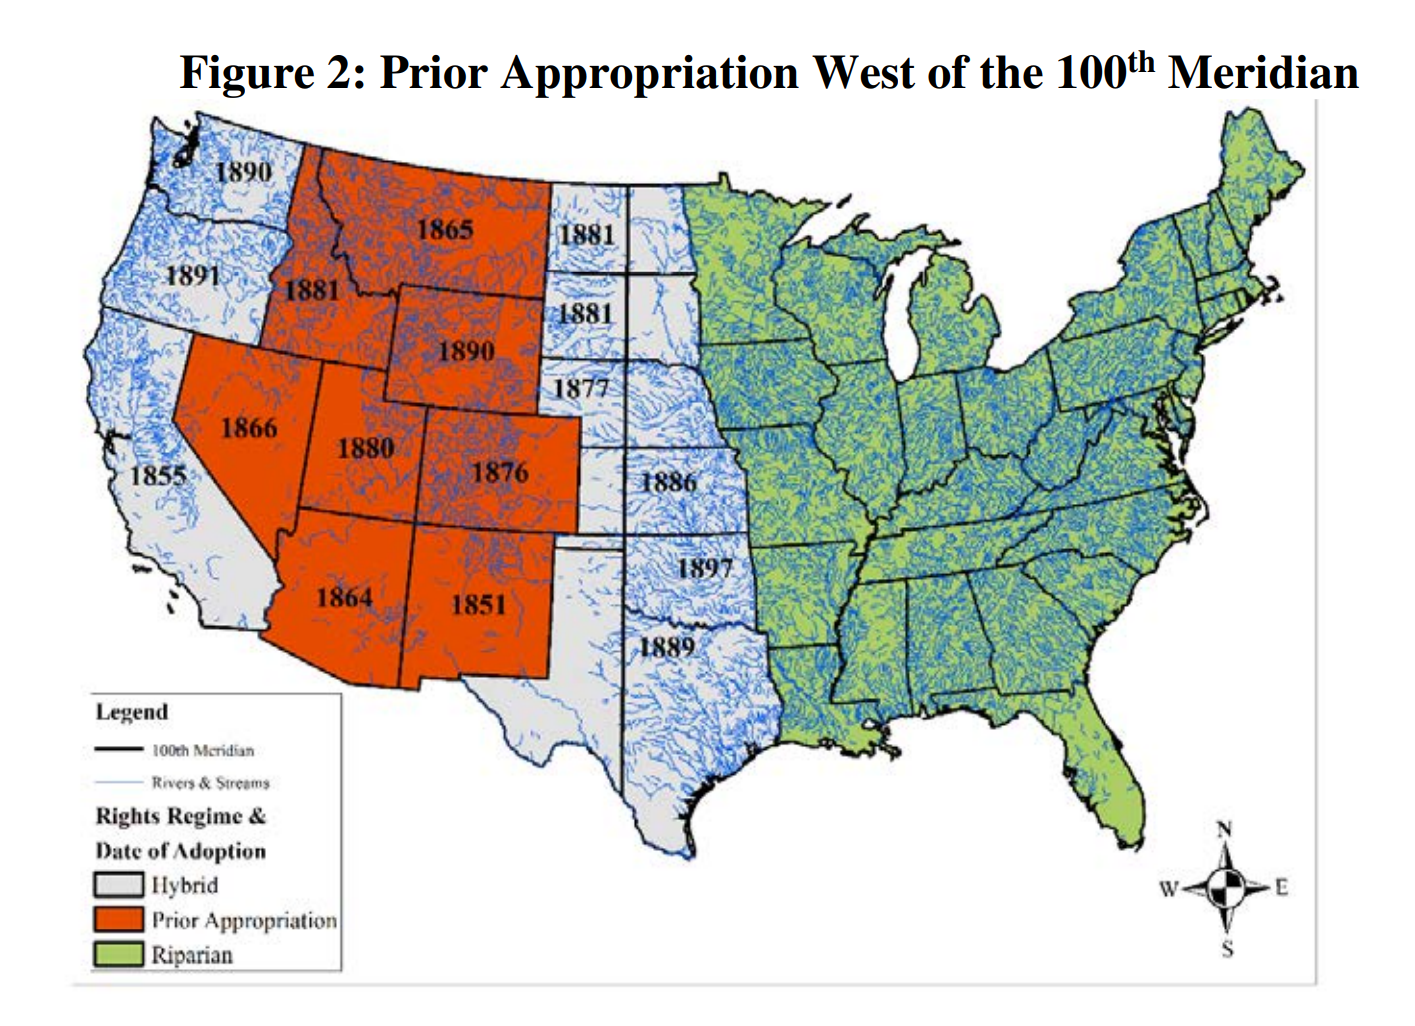
\includegraphics[width=\textwidth,height=4.16667in]{figures/m10_prior_appropriation_development.png}

\hypertarget{institutional-path-dependence}{%
\subsection{Institutional Path
Dependence}\label{institutional-path-dependence}}

\begin{itemize}
\tightlist
\item
  Path dependence: how events/decisions happened in the past may have
  long-run consequences, even though past circumstances may no longer be
  relevant
\item
  Our present is largely shaped by the historical critical junctures in
  institutional choices (Acemoglu and Robinson)

  \begin{itemize}
  \tightlist
  \item
    The Glorious Revolution
  \item
    World War II
  \item
    Presidential term limits
  \end{itemize}
\item
  Prior appropriation is certainly one of the legacy institutions

  \begin{itemize}
  \tightlist
  \item
    Water infrastructure no long need coordination
  \item
    Creates winners \& losers
  \end{itemize}
\end{itemize}

\hypertarget{section-38}{%
\subsection{}\label{section-38}}

From your perspective, at what point (if any) does this discussion about
water rights break down or become irrelevant for the Western US?

\hypertarget{section-39}{%
\subsection{}\label{section-39}}

How do dramatic technical innovations fit into the economic assessment?
What is the probability of the implementation of approaches that are
currently considered `wild' (for example, piping water from Canada
and/or Alaska, large scale desalination factories and piping from the
west, etc). At what point (if ever) do these become feasible?

\hypertarget{wild-technologies}{%
\subsection{Wild technologies}\label{wild-technologies}}

\begin{itemize}
\tightlist
\item
  Desalination
\item
  Piping water from Canada/Alaska
\item
  Dragging Icebergs from the Arctic
\item
  Ship water from Minnesota
\end{itemize}

When will these become relevant?

\hypertarget{marginal-benefits-and-prices-for-water}{%
\subsection{Marginal benefits and prices for
water}\label{marginal-benefits-and-prices-for-water}}

\begin{longtable}[]{@{}lll@{}}
\toprule
Use & Marginal Benefit & Average Price\tabularnewline
\midrule
\endhead
Domestic & 1122 & 652\tabularnewline
Agriculture & 250 & 16\tabularnewline
\bottomrule
\end{longtable}

(Units: \$/Acre Foot)

\hypertarget{cost-of-wild-technologies}{%
\subsection{Cost of Wild technologies}\label{cost-of-wild-technologies}}

\begin{longtable}[]{@{}ll@{}}
\toprule
Technology & Cost (\$/acre feet)\tabularnewline
\midrule
\endhead
Surface water withdraw & \$4\tabularnewline
Pumping cost from Ogallala (scarcity rent included) &
\$300\tabularnewline
Carlsbad Desalination Plant & \$2000\tabularnewline
Dragging iceberg from Antarctica & \$2500 (?)\tabularnewline
Rail shipping from Minnesota to California & \$160,000\tabularnewline
\bottomrule
\end{longtable}

\hypertarget{other-solutions-to-water-scarcity}{%
\subsection{Other solutions to water
scarcity}\label{other-solutions-to-water-scarcity}}

\begin{itemize}
\tightlist
\item
  What are the potential ways to limit water use?
\item
  And who is the world's leading player in this?
\end{itemize}

\hypertarget{section-40}{%
\subsection{}\label{section-40}}

At the moment, there are clear winners and losers in the water rights
systems of the western states. What would happen to the system if a
technological solution were found (and implemented) that removed the
concern about water supply in the region?

\hypertarget{water-markets}{%
\subsection{Water Markets}\label{water-markets}}

\begin{itemize}
\item
\end{itemize}


\end{document}
